
\section{Fonament teòric}

Primerament, és interessant fer una distinció entre la diferencia d'una reentrada balística i una reentrada sustentadora. Aquests dos tipus de reentrada són àmpliament usats en les missions actuals i mentre que la sustentadora permet més flexibilitat en quant a control, la entrada balística suposa menys càlculs matemàtics.

\subsection{Entrada balística}
Una entrada balística es defineix com una reentrada atmosfèrica en què les úniques forces són la gravetat i la força \textit{Drag} aerodinàmic. En canvi, una reentrada no balística, \ie, \textit{entrada sustentador} introdueixen altres forces per intentar augmentar la durada de la reentrada i així disminuir la dissipació d’energia durant un període de temps més gran. 

L'energia mecànica que té un objecte en la reentrada és molt elevada:
\begin{equation}
    E_{\mathrm{mec}} = \frac{mv^2}{2} + GMm\left( \frac{1}{r_{\mathrm{earth}}} - \frac{1}{r}\right)
\end{equation}
Un dels principis fonamentals de la física és que l'energia en un sistema tancat es conserva. La pregunta és, on va a parar tota aquesta energia que conté? La resposta a aquesta pregunta és que tota l'energia acumulada es bescanvia amb l'aire en forma d'energia de fregament.


\subsubsection{El coeficient balístic}
L'equació del moviment es pot escriure com:
\begin{equation} \label{eq:aceleracio}
    \Vec{a} = \frac{1}{2}\rho V^2 \frac{C_D A}{m}
\end{equation}
Observant l'equació \ref{eq:aceleracio} el terme $\frac{C_D A}{m}$ té un sentit físic molt usat en l'estudi de les trajectòries balístiques. Aquest coeficient s'anomena coeficient balístic i té un significat especial en la descripció de com es mou un objecte en l'atmosfera i s'expressa de la següent manera:
\begin{equation}
    \beta = \frac{W}{C_D A}
\end{equation}
on 
$\beta$: coeficient balístic del vehicle ($\kg/\meter^2$)
$W$: pes del vehicle ($\newton$)
$C_D$: Coeficient de Resistència aerodinàmica ($\mathrm{adim}$)
$A$: Secció transversal del vehicle ($\meter^2$)

És precisament a partir d'aquesta expressió que es mostra que l'acceleració d'un objecte és inversament proporcional  al coeficient balístic $\beta$. En altres paraules, un objecte amb un baix coeficient balístic, desaccelera molt més ràpidament que un objecte amb un alt coeficient balístic.

El coeficient balístic és per tant el paràmetre més important en el control de la trajectòries en la reentrada. Com a conseqüència, les calor s is desacceleracions son menys intenses per un valor reduït de $\beta$ (baix pes i/o alta resistència aerodinàmica o àrea) que per un valor elevat de $\beta$ (gran pes i/o baix drag reduïda àrea). Tots aquests conceptes s'analitzaran en detall en la següents seccions [Veure Annex \ref{fig:ballistic_terrestre}] \cite{nasa_ballistic} \cite{nasa_vol_drag}.

\newpage
\subsection{Entrada sustentadora}
Recordem que l'entrada balística se suposava que la força de sustentació $L$ a la reentrada és nul·la. Tanmateix, si s'afegeix una força de sustentació a la reentrada, aquest aportarà més flexibilitat en quant al marge d'error a la velocitat de reentrada o angle de trajectòria. A més, aquest tipus de reentrada permet millorar la precisió. Alhora, també permet canviar l'angle d'atac per millorar la sustentació de tal forma que e vehicle adopti un comportament més d'aeronau que d'un objecte sòlid en caiguda.

No obstant, tot i que la resistència aerodinàmica és present durant tota la reentrada, la trajectòria resultant es pot ajustar contínuament per canviar ambdós moviments verticals i direcció de vol quan es redueix la velocitat. De la mateixa manera que per la reentrada balística, el coeficient més important és la $\beta$, en una reentrada sustentadora, el paràmetre de disseny primari és la eficiència aerodinàmica:
\begin{equation}
    \frac{L}{D} = \frac{C_L}{C_D}
\end{equation}
Valors reduïts de $L/D$ produeixen càrregues $g$ moderades, moderats nivells de calor i poca maniobrabilitat. En canvi, valors elevats d'eficiència aerodinàmica produeixen càrregues $g$ reduïdes, tanmateix, les entrades són de llarga duració i de transferència de calor contínua. En el cas del Space Shuttle, la eficiència aerodinàmica és de l'ordre de la unitat.

\begin{figure}[ht]
    \centering
    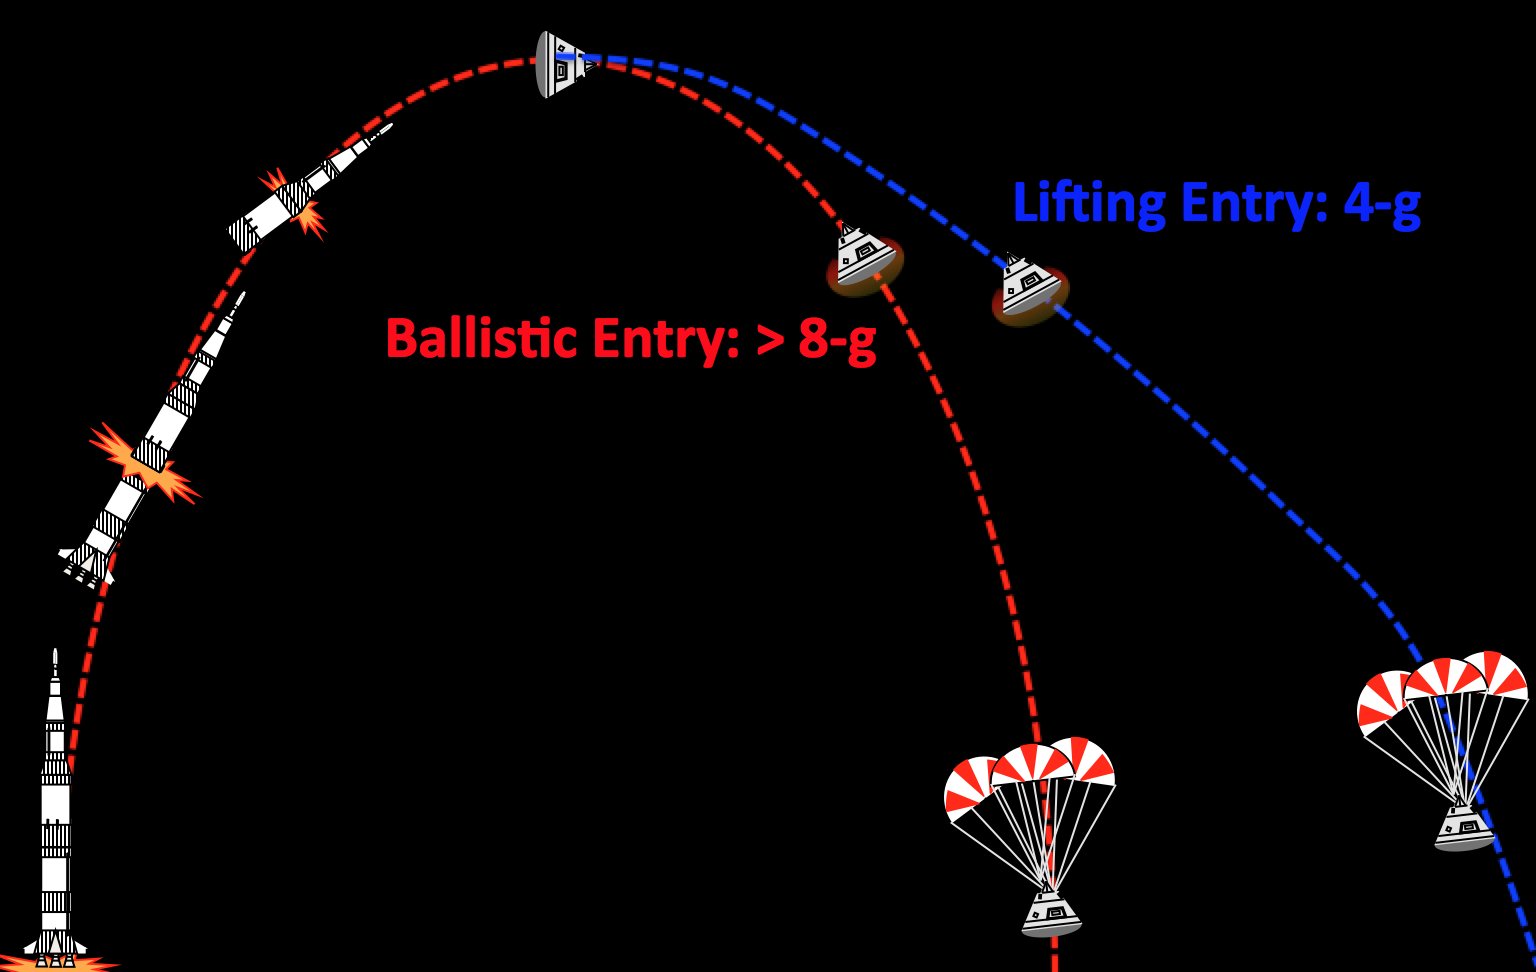
\includegraphics[width=0.5\textwidth]{imagenes/00_general/ballistic_vs_lifting.png}
    \captionsetup{width=0.6\textwidth}
    \caption{Comparació de la desacceleració entre entrada balística i l'entrada sustentadora. Crèdits: \cite{robert_frost}}
    \label{fig:ballistic_vs_lifting}
\end{figure}

\begin{figure}[ht]
    \centering
    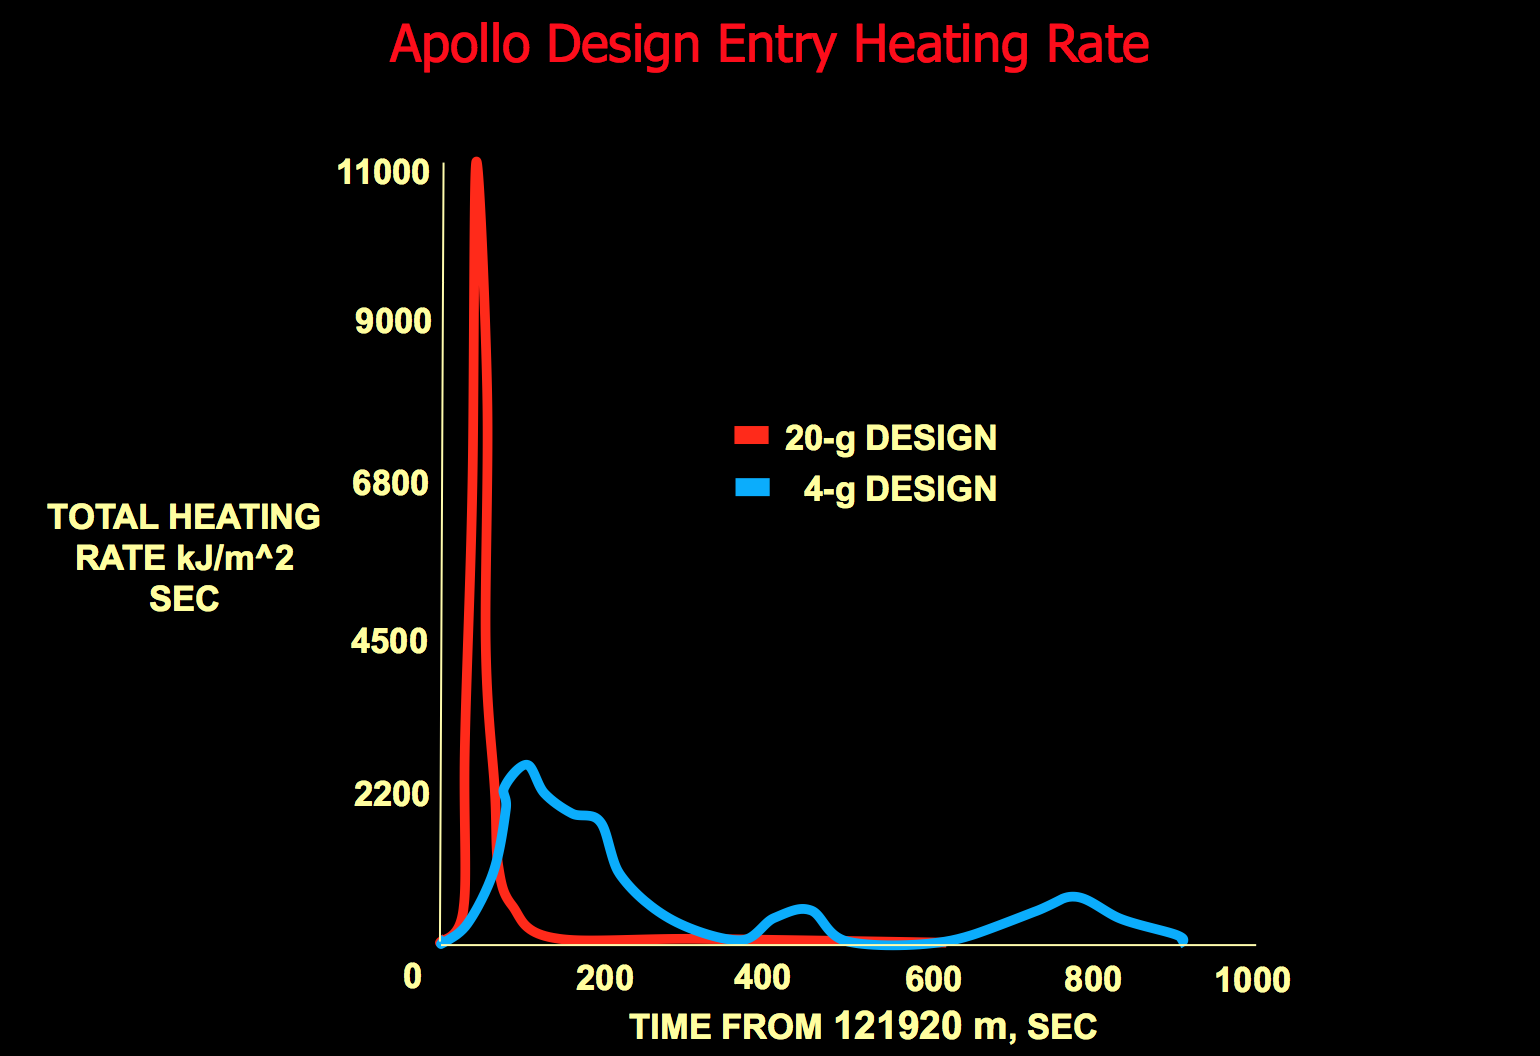
\includegraphics[width=0.5\textwidth]{imagenes/00_general/heating_ballistic_vs_lifting.png}
    \captionsetup{width=0.6\textwidth}
    \caption{Comparació de l'energia adquirida entre l'entrada balística i l'entrada sustentadora. Crèdits: \cite{robert_frost}}
    \label{fig:heating_ballistic_vs_lifting}
\end{figure}


\newpage
\subsection{Models d'atmosfera estàndard 1976 USA}
El model d'atmosfera estàndard internacional desenvolupat pels Estats Units d'Amèrica l'any 1976 es va construir a partir de la compilació de dades meteorològiques de l'hemisferi nord. L'estudi realitzat per John C. Adams, Jr. es basa en aquest sistema pel càlcul de les variables atmosfèriques tot i que el model GRAM de la NASA és el que actualment s'utilitza juntament amb el marc de l'atmosfera ISA (\emph{International Standard Atmosphere}). 

L'atmosfera USSMA inclou 14 atmosferes diferents corresponents a latituds que van des dels $15\degrees$ fins els $75\degrees$, per a diferents estacions (primavera/tardor, estiu/hivern) sempre per a altituds inferiors als $120 \ \kilo\meter$. A partir d'ara s'utilitzarà la latitud corresponent a $45\degrees$.

Aquest model utilitza una altura geopotencial $h$ que es defineix com:
\begin{equation}
    g_\mathrm{ref} h = \int_{0}^{z} g(z) \, \dd z 
\end{equation}
on $g(z)$ representa un valor aproximat del camp de gravetat a la latitud considerada a una altitud geomètrica $z$.
\begin{equation}
    g(z) \approx g(0) \frac{{R_t}^2}{(R_t+z)^2}
\end{equation}
on les expressions $R_t$ i $g(0)$ són també funcions de la latitud, que indiquen el radi terrestre i la gravetat de referència a nivell del mar, respectivament.

Atès que la atmosfera abasta una distància considerable, el perfil de pressió i temperatura varia considerablement entre les diferents capes que la composen. D'aquesta manera, a partir de la definició d'altura geopotencial:
\begin{equation}
    \dd p = -\rho g \, \dd z = -\rho g_\mathrm{ref} \, \dd z
\end{equation}
Una vegada combinada amb l'equació d'estat, s'obté:
\begin{equation} \label{eq:derpressio}
    \frac{\dd p}{p} = -\frac{M g_\mathrm{ref}}{R T} \, \dd h
\end{equation}
A continuació, s'integra l'equació \eqref{eq:derpressio} entre $h_b$ i $h$ per obtenir:
\begin{equation}
    p \left( h \right) = 
    p \left( h_b \right) \, 
    \exp{\left( \frac{M g_\mathrm{ref}}{R} \int_{h_b}^h \frac{\dd \mathit{h}}{T \left( \mathit{h} \right)} \right)}
\end{equation}
Prenent un model de temperatura lineal com
\begin{equation}
    T(h) = T_b + \lambda (h - h_b)
\end{equation}
on $\lambda$ és el gradient de temperatura a la capa, es poden distingir dos casos:
\begin{itemize}
    \item Per a capes atmosfèriques isotermes, \ie, amb $\lambda = 0$:
    \begin{equation}
        p(h) = 
        p \left( h _b \right) \exp{\left( - \frac{M g_\mathrm{ref}}{R T_b} \left( h - h_b \right) \right)}
    \end{equation}
    \item Per a capes atmosfèriques no isotermes:
    \begin{equation}
        p(h) = 
        p \left( h_b \right) 
        {\left( \frac{T_b + \lambda \left( h - h_b \right)}{T_b} \right)}^{-\frac{M g_\mathrm{ref}}{\lambda R}}
    \end{equation}
    \end{itemize}
Finalment, per al càlcul de la densitat:
\begin{equation}
    \rho(h) = \frac{M}{R} \cdot \frac{p(h)}{T(h)}
\end{equation}
Considerant com a constants conegudes en el cas de la Terra:
\begin{equation}
    M = 28.9644 \cdot 10^{-3} \quad \frac{kg}{mol}
\end{equation}
\begin{equation}
    g_{ref} = 9.80665 \quad {\frac{m}{s^2}}
\end{equation}
\begin{equation}
    p(0) = 101325 \quad Pa
\end{equation}
A continuació es presenten les diverses seccions de l'atmosfera terrestre que s'utilitzaran per a modelitzar les diverses variables termodinàmiques en funció de l'altura.

\begin{table}[ht]
    \centering
    \begin{tabular}{@{}cccc@{}}
        \toprule
        \multicolumn{4}{c}{\textbf{Altituds geopotencial i temperatura inicial a cada secció}} \\ \midrule
        \begin{tabular}[c]{@{}c@{}}Index de\\ secció\end{tabular} &
        \begin{tabular}[c]{@{}c@{}}Altituds\\ $h_{b} (m)$\end{tabular} &
        \begin{tabular}[c]{@{}c@{}}Gradients\\ $A_{b} (\frac{K}{m})$\end{tabular} &
        \begin{tabular}[c]{@{}c@{}}Temperatures\\ $T_{b} (K)$\end{tabular} \\ \midrule 
        1            & 0.                & -6.5$ \cdot 10^{-3}$              & 288.15          \\
        2            & 11000.            & 0.                                & 216.65          \\
        3            & 20000.            & +1. $\cdot 10^{-3}$               & 216.65          \\
        4            & 32000.            & +2.8 $\cdot 10^{-3}$              & 228.65          \\
        5            & 47000.            & 0.                                & 270.65          \\
        6            & 52000.            & -2 $\cdot 10^{-3}$                & 270.65          \\
        7            & 61000.            & -4 $\cdot 10^{-3}$                & 252.65          \\
        8            & 69000.            & -3 $\cdot 10^{-3}$                & 220.65          \\
        9            & 79000.            & 0.                                & 190.65          \\
        10           & 90000.            & +2 $ \cdot 10^{-3}$               & 190.65          \\
        11           & 100000.           & +4.36 $\cdot 10^{-3}$             & 210.65          \\
        12           & 110000.           & +16.4596 $\cdot 10^{-3}$          & 254.25          \\
        13           & 117776.           &                                   & 382.24          \\ 
        \bottomrule
    \end{tabular}
    \caption{A partir de \cite{gallais}.}
    \label{tab:altituds}
\end{table}
\noindent
A partir d'aquestes dades es deriven els següents paràmetres \cite{gallais}:
\begin{itemize}
    \item Velocitat del so:
    \begin{equation}
        a = \sqrt{\gamma \frac{R}{M} T}
    \end{equation}
    amb $\gamma = C_p / C_v$ i $r= R / M_m =287.053 \ \joule/ \left( \kilo\gram \, \kelvin \right)$.
    \item Viscositat dinàmica (Sutherland):
    \begin{equation}
        \mu = \frac{B \, T^{3/2}}{T+S}
    \end{equation}
    amb $B = 1.458 \cdot 10^{-6} \ \kilo\gram / \left( s \, \meter \, \kelvin^{1/2} \right)$ i $S = 110.4 \ \kelvin$.
\end{itemize}














